\chapter{Outsider Anonymous Identity-Based Broadcast Encryption}
\label{cha:n}

\section{Online Social Network}
OSNs are getting more and more aware of the rising privacy concerns among their users. Therefore, most OSN services like Google+ and Facebook try to offer preferences that allow the user to determine their privacy up to a certain extent. In practice, most OSNs realise this by offering user specified groups of friends that can be selected when broadcasting a message over the OSNs' network. The OSN provider then ensures that the broadcasted message is only shown to members inside the user specified group.

\subsection{Definition}
It might be useful to take one step back and define what an online social network actually is. Different definitions have found their way in literature but the most commonly accepted is the definition of a \textit{Social Networking Service} (SNS) from Boyd et al~\cite{art:BoydE08}.

\begin{defn}[Definition of a SNS by Boyd et al~\cite{art:BoydE08}]
\label{def:osn_boyd}
 A \textit{social networking service} (SNS) is a web-based service that allows individuals to:
 \begin{enumerate}
  \item Construct a public or semi-public profile within a bounded system
  \item Articulate a list of other users with whom they share a connection.
  \item View and traverse their list of connections and those made by others within the system
  \setcounter{enumTemp}{\theenumi}
 \end{enumerate}
\end{defn}

Definition~\ref{def:osn_boyd} is at the same time generic enough to cover all kinds of social networking services, as well as specific enough to distinguish SNSs from other web-based applications. However, Definition~\ref{def:osn_boyd} is still too generic for our purposes as we only consider one specific type of SNS, namely the SNSs from Definition~\ref{def:osn_boyd} that offer the ability to broadcast messages. Therefore, an \textit{Online Social Network} (OSN) is redefined in Definition~\ref{def:osn}. For the sake of clarity, from this moment onwards SNS will refer to a Social Networking Service as in Definition~\ref{def:osn_boyd} while OSN will denote an Online Social Network as in Definition~\ref{def:osn}.

\begin{defn}[OSN]
\label{def:osn}
 An \textit{Online Social Network} (OSN) is a social networking service (SNS), that in addition to the possibilities from Definition~\ref{def:osn_boyd} also allows its users to
 \begin{enumerate}
  \setcounter{enumi}{\theenumTemp}
  \item Distribute messages to anyone visiting the system, any user of the system or subsets thereof.
 \end{enumerate}
\end{defn}


\subsection{Model}

\begin{defn}[OSN user]
\label{def:user}
 An \textit{OSN user} $U$ is any entity that has a profile on the OSN and thus identifiable by a unique identifier \id{U}. The set containing all users of an OSN is denoted $\mathcal{U}$.
\end{defn}

An OSN user can perform different activities within the infrastructure of the OSN. Depending on the performed activity, the user is labeled as one of three different roles: a sender, a friend or a recipient.

\begin{defn}[Sender]
\label{def:sender}
 A \textit{sender} $B$ is an OSN user who broadcasts a message $m$ over the OSN infrastructure to varying subsets of OSN users, called the \textit{intended recipient set} $\mathcal{S}$ such that $\mathcal{S} \subseteq \mathcal{U}$.
\end{defn}

\begin{defn}[Intended recipient]
\label{def:recipient}
 An \textit{intended recipient} $R$ of a message $m$ is an OSN user who is explicitly designated by a sender $B$ to be part of the intended recipient set $\mathcal{S}$ of that message $m$.
\end{defn}

\begin{defn}[Friend]
\label{def:friend}
 An OSN user who shares a connection with another OSN user $U$ in the OSN infrastructure, is called a \textit{friend of the user $U$}. The set of all friends associated to a user $U$ is denoted $\mathcal{F}_U$ such that $\mathcal{F}_U \subseteq \mathcal{U}$.
\end{defn}

Currently, other entities than OSN users $U \in \mathcal{U}$ associated with a profile $\id{U}$, can access the OSN services as well. Therefore, it is required to define another group of entities called \textit{the viewers}.

\begin{defn}[Viewer]
\label{def:viewer}
 Any virtual or real world entity that is given access to the OSN belongs to the set of viewers $\mathcal{V}$. All viewers with access to the profile $\id{U}$ of a user $U$ are in the set $\mathcal{V}_U \subseteq \mathcal{V}$.
\end{defn}

In modern day OSN infrastructures, many different entities are part of the set of viewers $\mathcal{V}$, i.e. OSN users, advertising companies, system administrators of the OSN, software applications specifically developed for the OSN, etc. Note that these entities do not have to be users neither real life persons. Companies or software code can be part of the set of viewers $\mathcal{V}$ as well. Usually, the OSN determines which entities are member of the set of viewers $\mathcal{V}$. Therefore, the user often has no control in who is a member of $\mathcal{V}_U$. That is, the user $U$ can not determine which entities have access to his profile $\id{U}$.

Figure~\ref{fig:current_model} illustrates previous definitions applied to an OSN as it is often encountered on the internet. The different sets in Figure~\ref{fig:current_model} are defined as follows:
\begin{itemize}
 \item The intended recipient set,
 \begin{equation*}
  \mathcal{S} = \{ \textrm{Recipient 1}, \textrm{Recipient 2} \}
 \end{equation*}
 \item The set of friends of user $B$,
 \begin{equation*}
  \mathcal{F}_B = \{ \textrm{Recipient 1}, \textrm{Recipient 2}, \textrm{Friend 1}, \textrm{Friend 2} \}
 \end{equation*}
 \item The set of viewers who have access to the profile of user $B$,
 \begin{equation*}
  \mathcal{V}_B = \{ \textrm{Recipient 1}, \textrm{Recipient 2}, \textrm{Friend 1}, \textrm{Friend 2}, \textrm{Sender } B, \textrm{Advertiser 1}, \textrm{Application 1} \}
 \end{equation*}
 \item The set of entities with access to the OSN,
\begin{equation*}
\begin{split}
 \mathcal{V} = \{ \textrm{Recipient 1}, \textrm{Recipient 2}, \textrm{Friend 1}, \textrm{Friend 2}, \textrm{Sender } B, \textrm{Advertiser 1}, \textrm{Application 1}, \\
 \textrm{User 1}, \textrm{User 2}, \textrm{Advertiser 2}, \textrm{Application 2} \}
\end{split}
\end{equation*}
\item The set of all users in the OSN,
\begin{equation*}
 \mathcal{U} = \{ \textrm{Recipient 1}, \textrm{Recipient 2}, \textrm{Friend 1}, \textrm{Friend 2}, \textrm{Sender } B, \textrm{User 1}, \textrm{User 2}\}
\end{equation*}
\end{itemize}


\begin{figure}[ht]
    \begin{center}
    \scalebox{0.78}{
        \begin{tikzpicture}[auto, node distance=-2mm, align=center,
            block/.style={rectangle,text width=6em,text centered,minimum height=9mm},
            line/.style={draw,very thick, ->},
            line2/.style={draw,very thick, <->},
            leg/.style={text centered},
            ]
            % Recipient set polygon
            \draw[dashed,color=cyan] (3.5,4) -- (8.5,4) -- (8.5,1.75) -- (3.5,1.75) -- (3.5,4);
            % Friends polygon
            \draw[dashed] (3,4.5) -- (9,4.5) -- (9,-0.25) -- (3,-0.25) -- (3,4.5);
            % Viewers Polygon
            \draw[dashed] (-5,5) -- (9.5,5) -- (9.5,-0.75) -- (-5,-0.75) -- (-5,5);
            % OSN Polygon
            \draw[dashed] (-5.5,5.5) -- (10,5.5) -- (10,-2.75) -- (-5.5,-2.75) -- (-5.5,5.5);
            %\draw[help lines] (-6,-5) grid (8,6);
            \path
                % Images
                (0,3) node [block] (pkg) {
\includegraphics[scale=0.15]{img/bluepkg.png}}
                (-4,3) node [block] (alice) {
\includegraphics[scale=0.15]{img/bluealice.png}}
                (5,3) node [block] (bob) {
\includegraphics[scale=0.15]{img/bluebob.png}}
                (7,3) node [block] (bob1) {
\includegraphics[scale=0.15]{img/bluebob.png}}
                (5,1) node [block] (bob2) {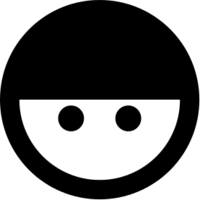
\includegraphics[scale=0.15]{img/bob.png}}
                (7,1) node [block] (alice1) {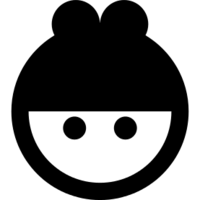
\includegraphics[scale=0.15]{img/alice.png}}
                (-1.5,1) node [block] (adv) {
\includegraphics[scale=0.15]{img/bluemoneyman.png}}
                (1.5,1) node [block] (app) {
\includegraphics[scale=0.15]{img/blueapp.png}}
                
                (1.5,-1.5) node [block] (app2) {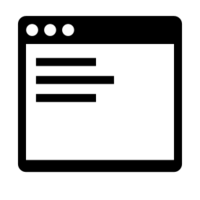
\includegraphics[scale=0.15]{img/app.png}}
                (-1.5,-1.5) node [block] (adv2) {
\includegraphics[scale=0.15]{img/moneyman.png}}
                
                
                (5,-1.5) node [block] (alice2) {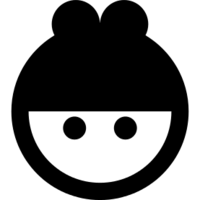
\includegraphics[scale=0.15]{img/alice.png}}
                (7,-1.5) node [block] (bob3) {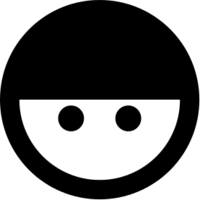
\includegraphics[scale=0.15]{img/bob.png}}
                
                (-1.5,-4) node [block] (spy1) {
\includegraphics[scale=0.15]{img/spy.png}}
                (1.5,-4) node [block] (spy2) {
\includegraphics[scale=0.15]{img/spy.png}}
                % Text
                (0,5.5) node [leg,fill=white] (white_block) {Entities with access to the OSN $\mathcal{V}$}
                (0,5) node [leg,fill=white] (white_block) {Entities with access to $B$'s Profile $\mathcal{V}_B$}
                (6,4) node [color=cyan,leg,fill=white] (white_block) {Intended Recipient Set $\mathcal{S}$}
                (6,4.5) node [leg,fill=white] (white_block) {Friends Set $\mathcal{F}_B$}
                (-2,3.25) node [leg,color=cyan] (white_block) {$m, \mathcal{S}$}
                ;
                
       \node[node distance=2mm, above=of pkg,color=cyan] {\textbf{OSN Server}};
       \node[below=of adv,color=cyan] {Advertiser 1};
       \node[below=of adv2] {Advertiser 2};
       \node[below=of app2] {Application 2};
       \node[below=of alice2] {User 1};
       \node[below=of bob3] {User 2};
       \node[below=of bob,color=cyan] {Recipient 1};
       \node[below=of bob1,color=cyan] {Recipient 2};
       \node[below=of bob2] {Friend 1};
       \node[below=of alice1] {Friend 2};
       \node[below=of app2] {Application 2};
       \node[below=of alice,color=cyan] {Sender $B$};
       \node[below=of app,color=cyan] {Application 1};
       \node[node distance=-6mm,below=of spy1] {Outsider 1};
       \node[node distance=-6mm,below=of spy2] {Outsider 2};
       \begin{scope}[every path/.style=line,color=cyan]
        \path (alice.east) -- (pkg.west);
        %\path (pkg.south west) -- (adv.north);
        \path (-0.7, 2.3) -- (adv.north);
        \path (0.7,2.3) -- (app.north);
        \path (pkg.east) -- (3.5,3);
       \end{scope}


        \end{tikzpicture}
    }
    \end{center}
    \caption{Model of the current OSN situation}
    \label{fig:current_model}
\end{figure}

Figure~\ref{fig:current_model} illustrates the situation in which Sender $B$ wants to broadcast a message over the OSN infrastructure to the intended recipient set $\mathcal{S}$. As Sender $B$ only wants to share her message with a specific group of friends, she defines the intended recipient set such that $\mathcal{S} \subset \mathcal{F}_B$. Next, she sends 

\subsection{Problem Statement}

\subsection{Existing Solutions}

\section{Security Model}

\subsection{Threat Model}

\subsection{Goals}

\section{Proposed Scheme}

\subsection{Scheme}

\subsection{Security Proof}

\subsection{Evaluation}

\section{Conclusion}

%%% Local Variables: 
%%% mode: latex
%%% TeX-master: "thesis"
%%% End: 
